\usemintedstyle{tango}
\setminted[python]{fontsize=\footnotesize, breaklines}
In the first part of this thesis we have established a theoretical basis about multigrid methods, formal languages and genetic programming.
In Chapter~\ref{chapter:multigrid-formal-language}, building on this foundation, we have then developed a novel formal language and grammar for the automatic generation of multigrid methods. 
While we have already demonstrated that the capabilities of this approach in alternating each individual step of a multigrid method, we could not yet demonstrate its benefits compared to the use of classical multigrid cycles, such as V-, F- and W-cycles.
We aim to achieve this goal with the implementation of \emph{EvoStencils}, a prototypical Python framework for the grammar-guided optimization of multigrid methods.
Using this framework we will then show how it is possible to evolve methods that are more efficient than all common multigrid cycles in solving a number of PDE-based problems while being structurally different that any other known method of this type.
However, before we discuss EvoStencils' features and their implementation in Python, we want to provide an overview about its workflow and software architecture.
In general, we can distinguish between EvoStencils' core implementation and the functionality of the framework that is build upon the use of external libraries.
First of all, since our formulation of the rules to construct a multigrid methods in the form of a context-free grammar, we can utilize the grammar-guided genetic programming techniques presented Chapter~\ref{chapter:formal-languages-and-gp} without adapting their inner workings.
For this purpose, we employ the widely-used evolutionary computation framework DEAP\footnote{DEAP: \url{https://github.com/deap/deap}}~\cite{rainville2012deap}, which enables us to implement GGGP in a modular way while requiring only a limited amount of adaption.
However, the questions that then remains to be answered how we can evaluate each multigrid method obtained through GGGP in an automatic and reproducible manner.
As we have seen in Section~\ref{sec:grammar-based-algorithm-generation} the 
application of the sequence of state transition functions represented in a given derivation tree produces a computational graph of the form of Figure~\ref{fig:example-three-grid-method-computational-graph}, which can then be transformed to an algorithmic representation, as shown in Algorithm~\ref{alg:example-three-grid-method-generated}.
However, while any expert could now manually implement the corresponding multigrid solver based on this representation using an arbitrary numerical software package, within GGGP we have to evaluate each method in an automatic way without requiring any human intervention.
Recently, code-generation techniques based on the specification of a numerical solver in a high-level domain specific language (DSL) have become increasingly powerful~\cite{kostler2020code}.
An example for this approach is the ExaStencils framework~\cite{lengauer2020exastencils,lengauer2014exastencils}, which has been specifically designed for the automatic generation of fast and scalable implementation of multigrid-based solvers specified in a tailored DSL called ExaSlang~\cite{schmitt2014exaslang,schmitt2016systems,kuckuk2016automatic}.
ExaSlang enables the formulation of a multigrid method as a sequence of high-level operations, without the need to consider the implementation details of each individual statement, while still granting the user the flexibility to apply further optimizations through the addition of code transformations and lower-level statements.
To evaluate a given solver, obtained from a grammar-based representation, we, therefore, emit its corresponding algorithmic formulation as an ExaSlang specification, based on which we then employ the ExaStencils framework to generate a scalable C++ implementation.
The resulting program can then be executed on a number of test cases in order to measure the desired performance characteristics of the solver.
Finally, note that the execution of a GGGP-based optimization approach requires the evaluation of a large number of different multigrid methods.
Depending on the problem that one aims to solve it can be infeasible to perform the optimization on a single compute node, necessitating the implementation of a multi-node parallelization.
The message passing interface (MPI)~\cite{walker1996mpi} provides a unified interface for performing parallel computations on a distributed system that is supported by the majority of supercomputing devices available.
While MPI has been originally designed for the traditional scientific computing languages Fortran and C, it recently has been also made available within Python~\cite{dalcin2021mpi4py}. 
With the addition of MPI, as a distributed computing backend, we arrive at the following high-level view of EvoStencils' software architecture, which is shown in Figure~\ref{fig:evostencils-architecture}.
\begin{figure}
	\resizebox{\columnwidth}{!}{%
		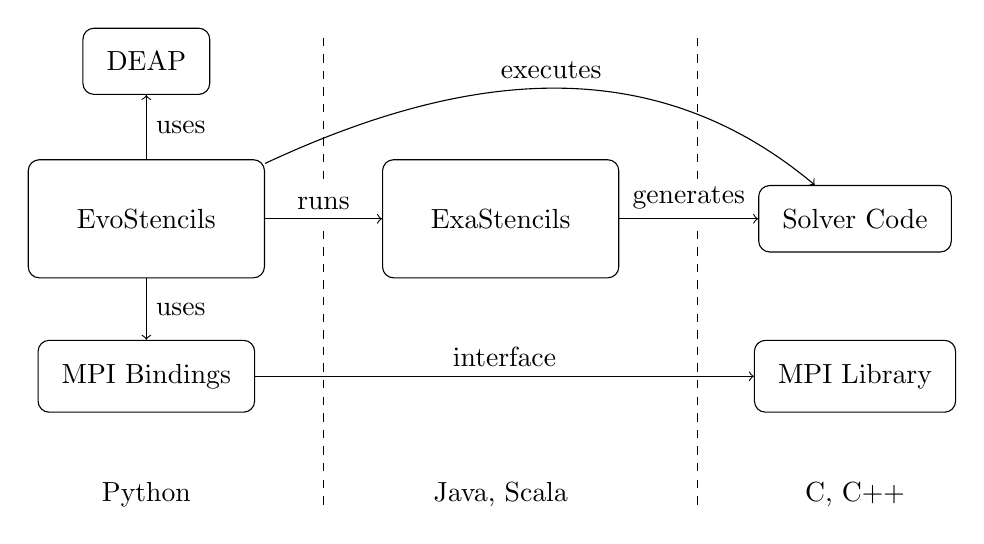
\begin{tikzpicture}
			%\draw [help lines] (-10,-10) grid (10,10);
			\node[draw, minimum width=3cm, minimum height=1.5cm, rounded corners] (evo) at (0,0) {EvoStencils};
			\node[draw, inner sep=3mm, rounded corners] (bindings) at (0, -2) {MPI Bindings};
			\node[draw, inner sep=3mm, rounded corners] (deap) at (0, 2) {DEAP};
			\node[draw, minimum width=3cm, minimum height=1.5cm, rounded corners] (exa) at (4.5, 0) {ExaStencils};
			\node[draw, inner sep=3mm, rounded corners] (code) at (9, 0) {Solver Code};
			\node[draw, inner sep=3mm, rounded corners] (mpi) at (9, -2) {MPI Library};
			\draw[dashed] (2.25, 2.3) -- (2.25,0.5);
			\draw[dashed] (2.25, -0.15) -- (2.25,-3.7);
			\draw[dashed] (7, 2.3) -- (7,0.5);
			\draw[dashed] (7, -0.15) -- (7,-3.7);
			\node (python) at (0, -3.5) {Python};
			\node (java) at (4.5, -3.5) {Java, Scala};
			\node (c) at (9, -3.5) {C, C++};
			\draw[->] (evo)-- node[anchor=west] {uses} (deap);
			\draw[->] (evo)-- node[anchor=south]{runs} (exa);
			\draw[->] (exa)--node[anchor=south] {generates} (code);
			\draw[->] (evo) to [out=25,in=140] node[anchor=south] {executes} (code);
			\draw[->] (bindings)--node[anchor=south] {interface}(mpi);
			\draw[->] (evo)--node[anchor=west] {uses}(bindings);
			%\draw[->] (mpi)--(code);
		\end{tikzpicture}
	}\caption{Software Architecture of EvoStencils.}
	\label{fig:evostencils-architecture}
\end{figure}
In the following, we will now consider the individual parts of this architecture in more detail, starting with the core implementation of EvoStencils, which can be considered as a separate module that does not depend on any of the other tools and libraries mentioned here.
As a first step, we will outline the implementation of an intermediate representation for multigrid methods that can be easily obtained from a given derivation tree and which then acts as a basis for all subsequent steps of solver generation and evaluation.

\section{Intermediate Representation}
Before we can represent the actual method and its computational structure, we need to be aware of the fact that all operations of a multigrid method are defined on a grid with certain step size.
Note that algebraic multigrid methods~\cite{stuben2001introduction,ruge1987algebraic}, which are not considered in this work, represent an exception to this, as they directly operate on sparse matrix and vector data structures.
In Section~\ref{sec:discretization} we have already made the assumption that we are able to discretize the underlying PDE on a hierarchy of structured grids.
Therefore, to identify a grid within this hierarchy certain information is required, which we store in a \texttt{Grid} data structure whose implementation is shown in Listing~\ref{code:ir:grid}.
In general a structured grid is identified by its size, i.e. the number of grid points, and spacing $h$ in each dimension.
In addition we also include the grid's level to identify it within the discretization hierarchy.
Note that in case the grid is uniform we only need to store a single value for the spacing in each dimension, while otherwise a value needs to be stored for each pair of grid points.
As the problems considered in this work are all solved on a hierarchy of uniform grids, we focus on this particular case.
However, whenever we apply this restriction it is clearly stated within the respective part of the code.  
\begin{listing}
	\inputminted{python}{evostencils/ir/grid.py}
	\caption{IR: Structure Grid}
	\label{code:ir:grid}
\end{listing}
After defining a data structure that provides all information about a certain grid within the discretization hierarchy, we can start defining expressions that operate on this data structure.
For this purpose, first in Listing~\ref{code:ir:abstact-base-class} a common abstract base class is provided from which all subsequent expression classes are derived.
\begin{listing}
	\inputminted{python}{evostencils/ir/expression.py}
	\caption{IR: Abstract Expression Base Class}
	\label{code:ir:abstact-base-class}
\end{listing}
In addition to the already mentioned grid data structure this class also defines a \texttt{shape} for each expression.
In a multigrid method each expression either computes a matrix or a vector.
For example, multiplying a $m \times n$-matrix with a $n \times m$-matrix yields a $m \times m$-matrix.
The shape of the corresponding expression is then defined as a pair $(r, c)$, whose first entry $r$ corresponds to the number of rows and the second $c$ to the number of columns, which in the given example is both $m$.
As in the case of matrix multiplication, the shape of each expression can always be derived from its operands, whose shape can be recursively determined in a similar manner.
Based on this abstract class, we can then further distinguish between predefined entities, such as the system matrix and right-hand side, and expressions that refer to the mathematical operations of a multigrid method.
First of all, Listing~\ref{code:ir:entity} contains the implementation of the entity base class.
\begin{listing}
	\inputminted{python}{evostencils/ir/entity.py}
	\caption{IR: Entity Base Class}
	\label{code:ir:entity}
\end{listing}
In addition to the previously mentioned properties, this class also contains a \texttt{name} to identify the respective entity.
Based on this implementation we can then further define classes for representing an approximate solution and right-hand side and operator, which are shown in the Listings~\ref{code:ir:approximation} and~\ref{code:ir:operator}.
\begin{listing}
	\inputminted{python}{evostencils/ir/approximation.py}
	\caption{IR: Approximate Solution and Right-Hand Side}
	\label{code:ir:approximation}
\end{listing}
\begin{listing}
	\inputminted{python}{evostencils/ir/operator.py}
	\caption{IR: Operator}
	\label{code:ir:operator}
\end{listing}
In both cases, the shape of the respective entity is obtained by computing the grid size product over all dimensions, whereas in case of the approximation and right-hand side the result can be considered as a vector while the shape of an operator corresponds to a quadratic matrix.
Note that as the \texttt{Approximation} and \texttt{RightHandSide} class, from a mathematical point of view, can be both considered as a vector, we only implement the former and then utilize inheritance to avoid unnecessary code duplication.
In addition to the attributes defined in its parent class, the \texttt{Approximation} includes a \texttt{predecessor} attribute, whose meaning will be discussed later within the implementation of grammar generation.
While the other two entities discussed here correspond to the solution and right-hand side of a discretized PDE, Listing~\ref{code:ir:operator} represents its operator, given in form of one or multiple stencil codes.
In Section~\ref{subsec:stencil-codes} we have already introduced a mathematical notation for stencil codes in form of Equation~\ref{eq:stencil-definition}, which can be implemented in the Python programming language in a straightforward manner that leads to the \texttt{Stencil} class shown in Listing~\ref{code:ir:stencil}.
%TODO introduce stencil implementation here
\begin{listing}
	\inputminted{python}{evostencils/ir/stencil.py}
	\caption{IR: Stencil}
	\label{code:ir:stencil}
\end{listing}
The \texttt{entries} attribute of this class directly corresponds to the set $S_h$ defined in Equation~\ref{eq:stencil-definition}, whereby we use a \texttt{tuple} object to represent this set in the Python programming language.
Each entry $e_i$ of this tuple then again represents a tuple of the form of
\begin{equation}
	e_i = \left(\bm{a}_i, b_i \right),
\end{equation} 
where $\bm{a}_i$ is the offset from the current grid point in each dimension, given as an array of integer values, and $b_i$ is the stencil value that corresponds to each offset, given as a floating point number.
Based on this class we can then provide implementations for all operations on stencil codes that have been defined in Section~\ref{subsec:stencil-codes}.
Furthermore, in accordance with Section~\ref{subsec:systems-of-pdes} and~\ref{subsec:block-smoothing}, we can extend this implementation to systems of PDEs and block smoothers, which will be briefly covered in the next Chapter of this thesis. %TODO insert ref to next chapter here or remove sentence
Now note that in our implementation of the \texttt{Operator} class in Listing~\ref{code:ir:operator} the stencil is not included directly, but instead we provide a so-called \emph{stencil generator}.
A stencil generator is a function that returns the instance of a certain stencil defined on a given grid, which enables us to obtain the corresponding stencil of a given discretized differential operator on different grids.
For instance, the Laplace operator $\nabla^2$ can be discretized on grids with different spacing and dimensionality.
Therefore, instead of storing a stencil for each individual problem instance, we can instead parametrize its generation based on the features of the applied discretization.

%TODO mention that we can not cover the full implementation here, refer to appendix
Additionally, the implementation of inter-grid operator classes can be found in the appendix.
Next, we need to provide classes for representing unary and binary expressions, which are shown in the Listings~\ref{code:ir:unary-expression} and~\ref{code:ir:binary-expression}.
\begin{listing}
	\inputminted{python}{evostencils/ir/unary_expression.py}
	\caption{IR: Unary Expression Base Class}
	\label{code:ir:unary-expression}
\end{listing}
\begin{listing}
	\inputminted{python}{evostencils/ir/binary_expression.py}
	\caption{IR: Binary Expressions Base Class}
	\label{code:ir:binary-expression}
\end{listing}
In both cases, all necessary properties are obtained from the expression's operands in a recursive manner.
However, as in case of a binary expression the shape of the result depends on the type of operation, we raise an error if this method is not implemented in one of the derived classes. 
While we will later see that there exist certain expressions that do not fall into these categories the majority of multigrid operations can be already expressed based on these two classes.
Again we have included a number of specific examples in the appendix.
As it has been discussed in Section~\ref{sec:grammar-based-algorithm-generation}, we aim to represent the computational structure of a given multigrid method in form of a redundancy-free directed graph. 
While the previously defined base classes allow us to represent the arithmetic expressions that occur within the correction terms of a multigrid method, there are two operations that require a special treatment.
As we have already seen in Figure~\ref{fig:example-three-grid-method-computational-graph} it is necessary to access previously computed intermediate results at multiple occasions within a multigrid method.
In particular, each time a coarse-grid correction is performed we have to restore the previous approximate solution and right-hand side on the respective level.
Furthermore, whenever we compute a new residual the current expression for both the right-hand side as well as the approximate solution are required.
For this purpose, we implement the classes \texttt{Residual} and \texttt{Cycle}, which serve the special-purpose of including additional references to previously defined expressions within a multigrid method.
Each of these references then corresponds to one of the subgraphs in Figure~\ref{fig:example-three-grid-method-computational-graph} whose root node possesses multiple incoming edges, i.e. the ones that have been annotated in Figure~\ref{fig:example-three-grid-method-computational-graph-annotated}.
We will later see how to utilize these references in order to construct a complete graph from the grammar-based representation of a multigrid method.
Listing~\ref{code:ir:residual} shows the implementation of the \texttt{Residual} class, which contains references to the system operator $A_H$, the expression for computing the current approximate solution $\tilde{x}_H$ and right-hand side $b_H$, where $H$ is the grid spacing on the current level.
Based on these components we can, thus, easily construct the corresponding residual expression $b_H - A_H \tilde{x}_H$.
\begin{listing}
	\inputminted{python}{evostencils/ir/residual.py}
	\caption{IR: Residual}
	\label{code:ir:residual}
\end{listing}
As a final step in the implementation of our intermediate representation, the definition of the \texttt{Cycle} class is shown in Listing~\ref{code:ir:cycle}.
\begin{listing}
	\inputminted{python}{evostencils/ir/cycle.py}
	\caption{IR: Multigrid Cycle}
	\label{code:ir:cycle}
\end{listing}
This class implements the functionality to represent a single step of multigrid cycle on a certain level with spacing $H$ with the purpose to compute a new value for the approximate solution $\tilde{x}_H$, i.e.
\begin{equation}
	\tilde{x}_H = \tilde{x}_H + \omega c_H \; \text{with} \; P,
\end{equation}
where $c_H$ is a correction term, $\omega$ the relaxation factor and $P$ a partitioning.
Furthermore, to make the right-hand side available to subsequent steps of the method, such as for the computation of the residual, we, again, need to include an additional reference into the data structure.
Finally, we also include a reference to the previous state on the next finer level, such that in case the result of a cycle is applied a coarse-grid correction, the previous expression for the approximate solution and right-hand side can be restored on that level.
To better understand the purpose of these two classes consider the following example shown in Listing~\ref{code:ir:example.py}, which demonstrate the construction of a computational graph based on the intermediate representation introduced in this section.
\begin{listing}
	\inputminted{python}{evostencils/ir/example.py}
	\caption{Example Usage of the Intermediate Representation}
	\label{code:ir:example.py}
\end{listing}
Starting on the original problem on the finest level, we first store references to the initial approximate solution and right-hand side in an \texttt{Cycle} object, which itself is included as a \texttt{predecessor} reference into the subsequently created coarse-grid \texttt{Cycle} object.
Finally, in order to apply the latter in form of a coarse-grid correction on the finest level, the original fine-grid \texttt{Cycle} object is restored and its \texttt{correction} variable is replaced by the respective expression which is obtained by prolongating the previously computed approximation on the coarse grid.
As this example demonstrate our intermediate representation (IR) enables us to construct the computational graph of a multigrid method in an iterative manner.
The next step towards the automatic generation of a multigrid method based on a grammar-based representation, now is to translate a sequence of derivations into the corresponding IR object.
For this purpose, we first have to consider how we can implement the formal system introduced in Section~\ref{sec:multigrid-grammar} using the functionality of the evolutionary computation framework DEAP~\cite{rainville2012deap}.
However, before we proceed with this discussion, we want to address some final remarks about the IR presented in this section.
First of all, note that while the main purpose of the implementation presented here is to uniquely represent the computational pattern of a multigrid method in form of a redundancy-free directed graph, in order to be able to construct this graph in a step-wise manner we have to include additional references into the respective nodes.
As we have shown in the previous discussion, the \texttt{Cycle} class serves this purpose by including additional information about the current state of a multigrid method, according to Definition~\ref{def:multigrid-state}, in form of references to the current approximate solution and right-hand side.
While this information is important for the construction of the graph, it could be later discarded by replacing each \texttt{Cycle} node with the respective arithmetic expression for computing an updated approximate solution, as it is shown in the \textsc{iterate} function in Section~\ref{sec:multigrid-state-transitions}.
However, preserving these additional references has the advantage of being able to easily traverse the sequence of \texttt{Cycle} nodes within each graph.
This does not only enable us to quickly grasp the computational structure of the corresponding multigrid method, but also facilitates the identification of potential errors in the implementation.
We, therefore, represent each newly computed approximate solution by an \texttt{Cycle} object, which is then referenced at each place of occurrence within subsequent computational steps of the method.
Also, note that even though the transformation of a graph-based to an algorithmic representation later requires us to translate each of these objects in a computational statement for updating the approximate solution, this operation can be performed while traversing the graph and, thus, does not induce a significant overhead within the process of algorithm generation. 
\section{Grammar Generation}
According to Section~\ref{sec:multigrid-grammar} our family of context-free grammar for the generation of multigrid methods consists of three components, a set of terminals, variables and productions, while additionally we have to choose a starting symbol $\ps{S}$ from the set of variables.
Furthermore, in Table~\ref{table:grammar-semantics} we have defined the semantics of each state transition function occurring within the productions listed in Table~\ref{table:multigrid-grammar}.
While Table~\ref{table:multigrid-grammar} fixes the number of coarsening steps, we have already seen that it is possible to define a similar grammar formulated on a different hierarchy of grid, for instance with a higher or lower number of coarsening steps.
We can, therefore, utilize this property to parametrize the generation of a grammar formulated on a particular hierarchy of grids with the employed number of coarsening steps.
For this purpose, we first need to generate the set of terminals that is defined on each level of the hierarchy, which is encapsulated into the class \texttt{Terminals} shown in Listing~\ref{code:grammar:terminals.py}.
\begin{listing}
	\inputminted{python}{evostencils/grammar/terminals.py}
	\caption{Terminals defined on each level.}
	\label{code:grammar:terminals.py}
\end{listing}
Note that this class comprises a few notable differences compared to our grammar formulation in Section~\ref{sec:multigrid-grammar}.
First of all, as, at least in the applications considered in this work, each smoother is derived directly from the system operator, it does not need to be provided explicitly, but instead can be generated automatically within the grammar.
Also, while so far we have abstractly represented the application of the coarse-grid solver in form of a multiplication with the inverse $A^{-1}_H$ on the coarsest level with spacing $H$, the coarse-grid solver itself can also be considered as a degree of freedom, to be provided by the user.
The implementation of this class can again be found in the appendix.
Note that the coarse-grid solver may additionally contain an expression, again given in form of an IR object representing a multigrid method.
This enables the construction of multigrid methods in a hierarchical manner, which means that after obtaining a multigrid method on a certain hierarchy of discretizations, we can employ it as a coarse-grid solver for those methods whose coarsest grid corresponds to its topmost level.
As a next step, based on the \texttt{Terminals} class, we can then implement the state transition functions shown in Table~\ref{table:grammar-semantics}, to construct the corresponding IR object of a multigrid method represented as a derivation tree of the grammar shown in Table~\ref{table:multigrid-grammar}.
From these components we will then finally be able assemble the actual grammar using the genetic programming module of the DEAP framework~\footnote{\url{https://deap.readthedocs.io/en/master/api/gp.html}}.
\begin{listing}
	\inputminted{python}{evostencils/grammar/residual_apply_iterate.py}
	\caption{}
	\label{code:grammar:residual-apply-iterate}
\end{listing}
\begin{listing}
	\inputminted{python}{evostencils/grammar/cocy_cgc.py}
	\caption{}
	\label{code:grammar:cocy-cgc}
\end{listing}


